\documentclass[10pt]{standalone}
\usepackage{ngerman, longtable}
\usepackage{amsmath}
\usepackage{amssymb}
\usepackage{fancyhdr}
\usepackage{pdflscape}
\usepackage{wasysym}
\usepackage{color}
\usepackage{longtable}
\pagestyle{fancy}
\usepackage{multirow}
\usepackage{array}
\usepackage{tikz}

\begin{document}
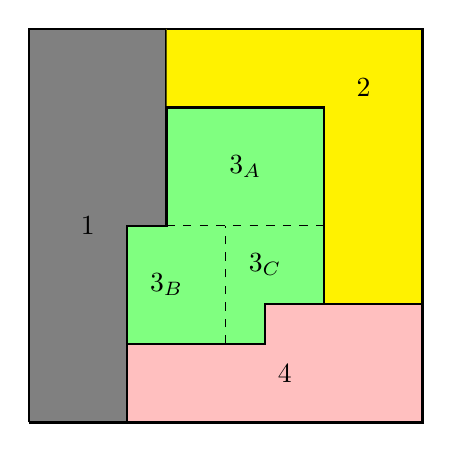
\begin{tikzpicture}[scale=5]
\coordinate (ll) at (0,0);
\coordinate (lr) at (1,0);
\coordinate (ul) at (0,1);
\coordinate (ur) at (1,1);

\coordinate (A) at (0.25,0);
\coordinate (B) at (0.35,0.5);
\coordinate (C) at (0.6,0.3);
\coordinate (D) at (0.6,0.4);
\coordinate (E) at (0.35,0.6);
\coordinate (F) at (0.75,0.3);
\coordinate (G) at (0.75,0.6);
%\node (a) at (A) {A};

% frame
\draw[black] (ll) -- (lr) -- (ur) -- (ul) -- (ll);
% left area
\draw[thick,black,fill=gray] (0,0) -- (0.25,0) -- (0.25,0.5) -- (0.35,0.5) -- (0.35,1) -- (0,1) -- (0,0);
\node (b1) at (0.15,0.5) {$1$};
% right lower area
\draw[thick,black,fill=pink] (0.25,0) -- (1,0) -- (1,0.3) -- (0.6,0.3) -- (0.6,0.2) -- (0.25,0.2) -- (0.25,0);
\node (c1) at (0.65,0.125) {$4$};
% upper right partitioned area
\draw[thick,black,fill=yellow] (0.35, 1) -- (1, 1) -- (1, 0.3) -- (0.75,0.3) -- (0.75, 0.8) -- (0.35, 0.8);
\node (d1) at (0.85,0.85) {$2$};

% middle partitioned area
\draw[thick,black,fill=green!50] (0.25,0.2) -- (0.6,0.2) -- (0.6,0.3) -- (0.75,0.3) -- (0.75,0.8) -- (0.35,0.8) -- (0.35,0.5) -- (0.25,0.5) -- (0.25,0.2);

% middle partitioned upper cluster area
\draw[thin, dashed, black,fill=green!50] (0.35,0.5) -- (0.75,0.5);
\node (a1) at (0.55,0.65) {$3_A$};

% middle partitioned left cluster area
\draw[thin, dashed, black,fill=green!50] (0.5,0.2) -- (0.5,0.5);
\node (a2) at (0.35,0.35) {$3_B$};
\node (a3) at (0.6,0.4) {$3_C$};

% \draw[step=0.1,black,ultra thin] (0.0,0.0) grid (1.0,1.0);

\end{tikzpicture}
\end{document}
